\subsection{System, communication and adversary model}%
\label{adversary-model}

We provide system model with three adversaries of varying strength.
We will start with the base model and then successively increase the 
adversary's strength.

\paragraph{The base malicious witness--storage model}

There are three players: the protest participant (with identity) \(P\), a 
witness (with identity) \(W\) and the storage \(S\).
The adversary \(A\) controls \(W\) and \(S\).

The protester \(P\) and the witness \(W\) communicate.
Each learn only the protocol data \(d_{P,W}(\cid, P)\) and when it happened 
\(t_{P,W}\), but specifically \emph{not} the real identities \(P\) and \(W\) 
directly --- only if it appears in the data \(d_{P,W}(\cid, P)\).
The protester \(P\) communicates with \(S\), where \(S\) only learns 
\(f(d_{P,W}(\cid, P))\), for some function \(f\), and the time of the 
communication (\(t_{P,S}\)) but not the real identities.
As the adversary controls \(W\) and \(S\) he learns everything that they do, 
but can additionally correlate what he learns from \(W\) and \(S\).

\begin{figure}
  \centering
  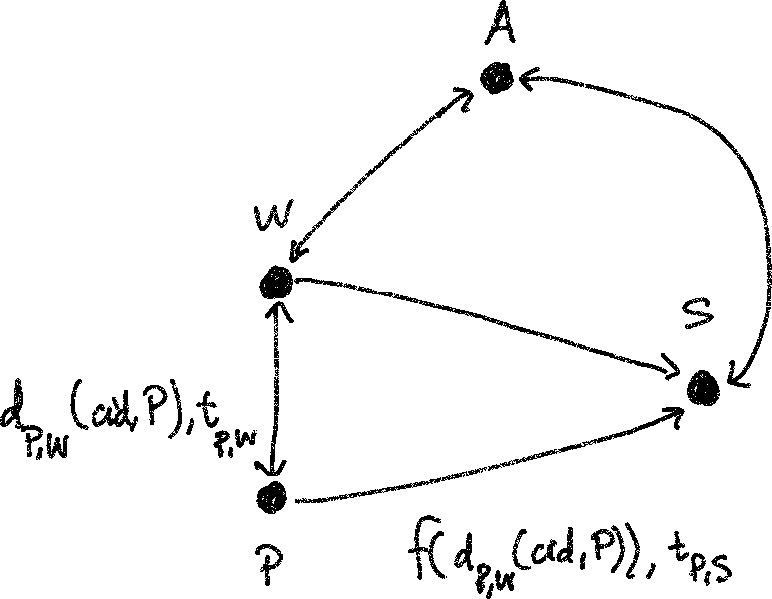
\includegraphics[width=\columnwidth]{system-model.png}
  \caption{\label{fig:system-model}%
    An overview of the system model.
    The protester with real identity \(P\) and witness with real identity \(W\) 
    communicate and each learn only the protocol data, \(d_{P,W}(\cid, P)\), 
    and the time it happened, \(t_{P,W}\).
    The protester submit some function of the protocol data \(f(d_{P,W}(\cid, 
      P))\) to the storage \(S\), who learns only that and the time it 
    happened, \(t_{P,S}\).
    Both the witness \(W\) and storage \(S\) are controlled by the adversary 
    \(A\).
  }
\end{figure}

\paragraph{The stronger malicious witness--storage model}

Now the witness \(W\) learns the protester \(P\)'s identity.
(\(P\) will also learn \(W\)'s identity.)
However, \(S\) still does not learn \(P\)'s identity.

\paragraph{The strongest malicious witness--storage model}

Now \(S\) also learns \(P\)'s identity.
